\chapter{Software Defined Networking} \label{chap:sdn} %% chapter 3

Computer networking is a vital part of the services that are offered today, and as such, the performance in technology backing these services is central to the quality of these services. As the service providers reorganize their
data centers in the cloud computing domain, enabling several improvements in the predictability, quality of service and ease of use of their services. New technologies are then required to make sure that their services are adapted
to the fast changing landscape of networking services. One of the most notable innovations in this field is called Software Defined Networking, because its architecture allows for two essential features

\begin {itemize}
    \item \textbf{Separation of network planes} SDN allows for the separation of the network control plane from the data forwarding plane by having network "intelligence" present in the network controllers, and having them
control the forwarding elements that live in the Data Plane
    \item \textbf{Centralization of network management functions} By isolating the management on a separate plane, there is possibility of developing a single controller that can regulate the entire network, having unrestricted access 
        to every element present in the network, simplifying management, monitoring, application of QoS policies, flow optimization, ...
\end {itemize}

\par This new paradigm introduces programmability in the configuration and management of networks, by consolidating the control of network devices to a single central controller, achieving separation of the control and the 
data plane, and supporting a more dynamic and flexible infrastructure. Another important paradigm, that follows the development of SDN, is the concept of Network Function Virtualization. This concept allows to remove 
\textit {middleboxes}\footnote {Computer networking device that does some operations on traffic, excepting packet forwarding. Examples include caches, IDS's, NAT's, ..}, by replacing these with generic software 
applications.

\par The essence of SDN is described in a short manner by the Open Networking Foundation (ONF), the maintainers of the OpenFlow protocol \ref{sec:of} paper: \textit{ In the SDN architecture, the control and data planes 
are decoupled, network intelligence and state are logically centralized, and the underlying network infrastructure is abstracted from the applications}. The following picture defines both of the approaches to networking,
the traditional one and the SDN way.

\begin{figure}[!tbph]
  \centering
  \subfloat[Traditional networking architecture]{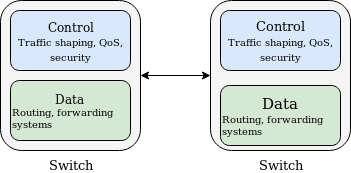
\includegraphics[width=0.4\textwidth]{bib/network_trad}\label{fig:net_trad}}
  \hfill
  \subfloat[SDN architecture]{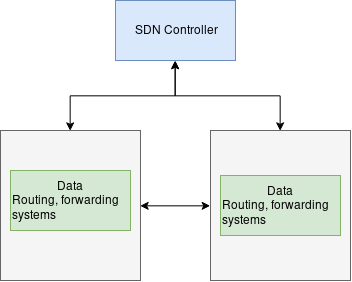
\includegraphics[width=.4\textwidth]{bib/network_sdn}\label{fig:net_sdn}}
  \caption {Traditional vs SDN network architecture}
\end{figure}

\par By moving network infrastructure to SDN models, the difficulty of managing a network is greatly reduced, since the logical centralization of the control layer exposes the global view of the network, simplifying tasks such as
setting forwarding rules. Furthermore, this also removes the challenge of configure each networking device individually, turning network operation and management into setting high level policies in the controllers, and letting 
the protocols that handle connection between the devices and controllers set the actual rules. It is then possible to define Software-Defined Networking as the composed of two layers: \textbf{Northbound Interfaces}, 
which are composed of Application Programming Interfaces (API) for communication between applications and the controller, enabling network services like routing, security, visualization and management; and the 
\textbf {Southbound Interfaces} which main role is to connect the network devices between the controllers and network via protocols like OpenFlow (see section \ref{sec:of}), or P4 \footnote {https://p4.org/}. 

\begin{figure}[!tbph]
  \centering
  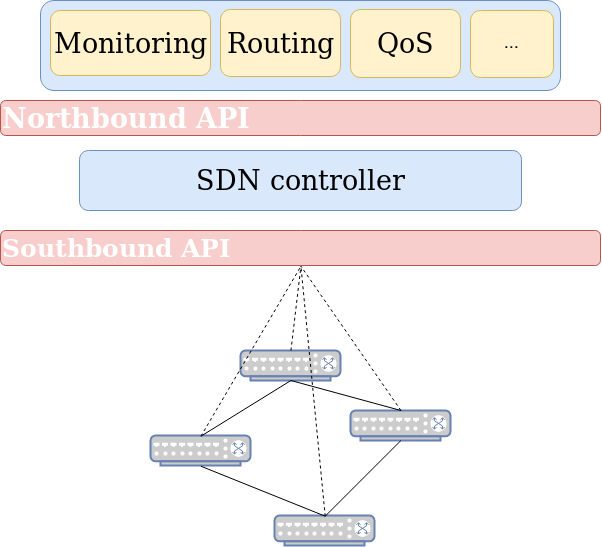
\includegraphics[width=0.4\textwidth]{sdn/sdn_division}
  \label{fig:sdn_div}}
  \caption {SDN Interfaces division}
\end{figure}

\par Understanding SDN platforms is then composed of understanding the operation of both interfaces, and defining requirements for their operation, which are listed below \cite {CITE - sdn_reference_architecture_open_api.pdf}.
These requirements are general principles for networks, but the addition of the SDN controller introduces another point of failure, that could be damaging to the entire network.

\begin {enumerate} 
    \itemsep0em
    \item High Performance   
    \item High Availability 
    \item Fault Tolerance   
    \item Monitoring   
    \item Programmability   
    \item Modularity   
    \item Security   
\end {itemize}

\section {OpenFlow} \label{sec:of}

As the growth of the networking infrastructure of the past few decades became evident, the need for an enviroment that allows for experimentation and testing of different protocols and equipment became evident. If networking 
research would depend on the previously existing methods, then new ways of creating and developing protocols would become increasingly hard to implement and develop. As such, there was need for a framework that could 
enable testing of new ideas on close to realistic settings. So, on February 2011 the version 1.1 of OpenFlow was released, and this proposal quickly became the standard for networking in a Software Defined Network. Since
2011, this protocol has suffered some revisions, and the latest version supported is version 1.5.1. Since this framework has evolved quite a bit, this section focuses on the versions 1.3, which are the versions that 
are used in development of this dissertation. 
\par Several reasons led to the quick standardization of this protocol, which are related not only to the initial requirements of the platform, like the capability of supporting high-performance and low-cost implementations, 
and the capability of ensuring separation between production and testing traffic, but also the extensibility that the open source development model provides, removing the limitations that closed or commercial solutions give the 
network researchers.
\par The big advantage of OpenFlow is that it is, from the data forwarding plane point of view, easy to process. Since the control decisions are made by the controller, which lives in a separate plane, all the switch needs to do
is correctly match the incoming packets, and forward them according to the rules established by the controller. The components that are part of this system and enable this functionality are:

\begin {itemize}
    \item \textbf {FlowTables} This element describes the main component of the switching capabilities of the OpenFlow switch. Inside the switch there are several flow tables that can be used to match incoming packets,
and process them in the rules that are specified by the controller. These rules can contain actions that affect the path of the packets, and these actions usually include forwarding to a port, packet modification, among
others. Classification is done via matching one or more field present in the packet, for example the switch input port, the MAC and IP addresses, IP protocol, basically all information required to correctly process the 
incoming packet. The required actions for an OpenFlow switch are the capability of forwarding to a set of output ports, allowing the packet to move across the network; to send them to the controller, in the case of a
miss of match; and finally the ability to drop packets, which is useful for DDoS mitigation, or more security concerns.
    \item \textbf {OpenFlow Protocol} Through the establishment of the OpenFlow Protocol between the switch and the controller, there is the definintion of several messages that allow for the control of the switch. This protocol
enables capabilities such as adding, deleting and updating flow mods in the switch, that are referred to as \textit {Controller-to-Switch} messages. Other relevant message types are the \textit {Asynchronous}, that enable the
notification of some event that occurred, this type includes the Packet-In message, that is a type of message that is sent to the controller when a certain packet has no match in the flow tables present in the switch; and the 
\textit{ Synchronous} message that enable functionality such as the Hello message, that is used to start the connection between the switch and the controller.
    \item \textbf {Secure Channel} OpenFlow defines the channel that is between the switch and the controller as a secure communications channel. As the messages that are sent to the switch are critical for the correct operation 
of the system, as indicated in the previous point, the channel should be cryptographically secure, to prevent spoofing of this information. As such, the channel is tipically transported over TLS.
\end {itemize}

% XXX SOURCE This images were taken from : open flow switch specification  https://3vf60mmveq1g8vzn48q2o71a-wpengine.netdna-ssl.com/wp-content/uploads/2014/10/openflow-switch-v1.3.5.pdf
\begin{figure} [h]
    \centering
    \begin{subfigure}
    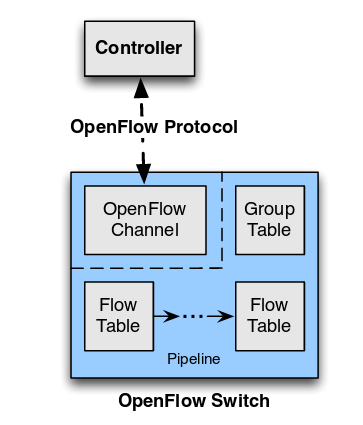
\includegraphics[width=0.25\textwidth]{sdn/open_flow_switch_pipeline}
    \end{subfigure}
    \begin{subfigure}
    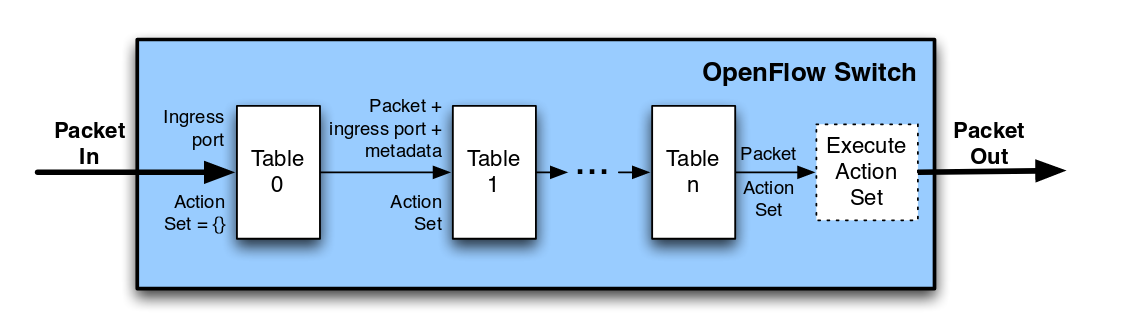
\includegraphics[width=0.6\textwidth]{sdn/open_flow_tables}
    \end{subfigure}
    \caption{Images describing OpenFlow components. On the left, an overview to the entire system, and on the right a view at the table structure of the OpenFlow Switch}
\end{figure}

\section {Network Devices} 

Networking devices are a central part of network operation, performing routing, switching, management operations, and span the different layers of the OSI model. The investment in dedicated hardware to perform management functions can
potentially be replaced by SDN controllers, offloading the QoS policies and traffic engineering (TE) functions from hardware to software. As such, in this section we focus on the devices that are responsible for the operation on 
layers 2 and 3 of the standardized networking stack, switches and routers. A networking switch is a device that connects multiple devices on a computer network, using hardware addresses (MAC) to forward data inside the network, 
by mapping each port with a certain MAC address, while a router is responsible of forwarding packets between different computer networks. These devices run at different layers of the networking stack, the former operating at the 
data-link, or layer 2, and the latter operating at layer 3, or network. This is not a clear separation however with multilayer devices, where switches also provide routing capabilities. Typical vendors for these solutions include
Cisco, Juniper, but the rise of whitebox switches that have support for deployments in SDN environments enables network operators to avoid vendor lock-in, and take advantage of the open nature of these devices. Commonly associated 
with whitebox switches is the support for the OpenFlow protocol, making these an essential part of the SDN infrastructures.

\par The performance \footnote {Defined as the throughput and latency of the network node} of networking devices is central to the proper operation of networks, especially in deployments in Data Centers, where the 
interfaces must be able to support 100 Gbps links and further, while also maintaining the programmability that is expected of SDN based infrastructures. This performance is linked with the hardware that is chosen to serve as the 
base for the devices \cite {CITE - sdn_challenges}:

\begin {enumerate} 
    \itemsep0em
    \item \textbf{General Purpose Processors} provide the greatest flexibility of all the solutions, while providing the worst results in performance, due to the general purpose design of the hardware and the optimizations present
        in the other architectures.
    \item \textbf{Field-Programmable gate arrays (FPGA)} are a platform that enable the configuration of the devices via hardware design tools, maintaining the programmability of the GPPs, while also allowing for designing the
        devices around the tasks that they perform, including optimizations for switching/ routing. A notable example of platforms based in these systems is NetFPGA \footnote {https://netfpga.org/site/\#/}, an open source 
        hardware platform designed for research, and supporting up to 100G operation. 
    \item \textbf{Application-specific integrated circuits (ASIC)} are integrated circuits that are customized for one particular application, removing the programmability, but also providing the greatest performance of the former 
        options.
\end {itemize}

\par These architectures generally allow to design SDN architectures around general purpose hardware, contributing to the flexibility of this paradigm, even considering the proprietary nature of the ASICs, which can be bundled with 
SDKs for developing other applications on top of these. 

\par Considering OF enabled hardware switches, the processing of incoming packets is done as by matching a (up to) 15 field tuple \cite {CITE - flow_table_management_sdn_switches} to several flow tables, 
that have rules sent from the controller. In these cases, the possibility of bottlenecks are due to several factors, including the latency of the installation of new flow rules, and the memory limitation on the hardware. Solutions 
to the memory limitations in OF switches include DevoFlow \cite {CITE - https://hal.inria.fr/hal-00825087/document}, which utilizes wildcard rules to reduce the number of flow entries that are installed on the devices, while also
aggregating traffic, which simplifies detection and management of the elephant flows, due to reduced control plane load; and SmartTime \cite {http://rishabhpoddar.com/publications/SmartTime.pdf} manages the timeouts
for the rules on the switch, reducing this in the presence of microflows, and increasing the timeout in the case of the occurrence of longer lived flows, which improves memory utilization and reduces the load on the controller.

\par Virtualised environments also allowed the development of Software Switches, due to the highly dynamic nature of virtual environments, where Virtual Machines (VMs) can move between physical compute nodes and frequent
network topology changes. Furthermore, standard Linux bridges cannot handle the multi-server deployments \footnote {https://github.com/openvswitch/ovs/blob/master/Documentation/intro/why-ovs.rst} used in virtualised environments. 
Open vSwitch is a soft switch that can join traditional switches on these platforms, replacing them where these couldn't be deployed. OVS switches are also compliant with the OpenFlow protocol, which clearly shows the flexibility
that can be achieved by combining all the networking devices with one management protocol. 

\section {SDN Controllers}

\subsection {Floodlight}
\subsection {OpenDaylight} \label{chap:odl}

